% Merkle lot commitment, two-layer label and on-chain consume checks, for one IEEE column (86 mm).
\documentclass[tikz,border=1pt]{standalone}
\usepackage{newtxtext,newtxmath}
\usetikzlibrary{arrows.meta,positioning,patterns}
\newcommand{\sm}{\fontsize{6}{7}\selectfont}
\newcommand{\md}{\fontsize{6.5}{7.6}\selectfont}
\newcommand{\qr}[2]{% #1 = centre, #2 = side (mm)
  \begin{scope}[shift={#1}]
    \fill[white] (-#2/2,-#2/2) rectangle (#2/2,#2/2);
    \foreach \x/\y in {0/0, 0.6/0.2, 0.2/0.6, 0.8/0.7, 0.45/0.45, 0.7/0.35, 0.3/0.15, 0.55/0.8}
      \fill (-#2/2+0.30*#2+\x*0.4*#2, -#2/2+0.30*#2+\y*0.4*#2) rectangle ++(0.09*#2,0.09*#2);
    \foreach \cx/\cy in {0/1, 1/1, 0/0} {
      \draw[line width=0.4pt] (-#2/2+\cx*0.72*#2+0.02*#2, -#2/2+\cy*0.72*#2+0.02*#2) rectangle ++(0.24*#2,0.24*#2);
      \fill (-#2/2+\cx*0.72*#2+0.08*#2, -#2/2+\cy*0.72*#2+0.08*#2) rectangle ++(0.12*#2,0.12*#2);
    }
  \end{scope}}
\begin{document}
\scriptsize
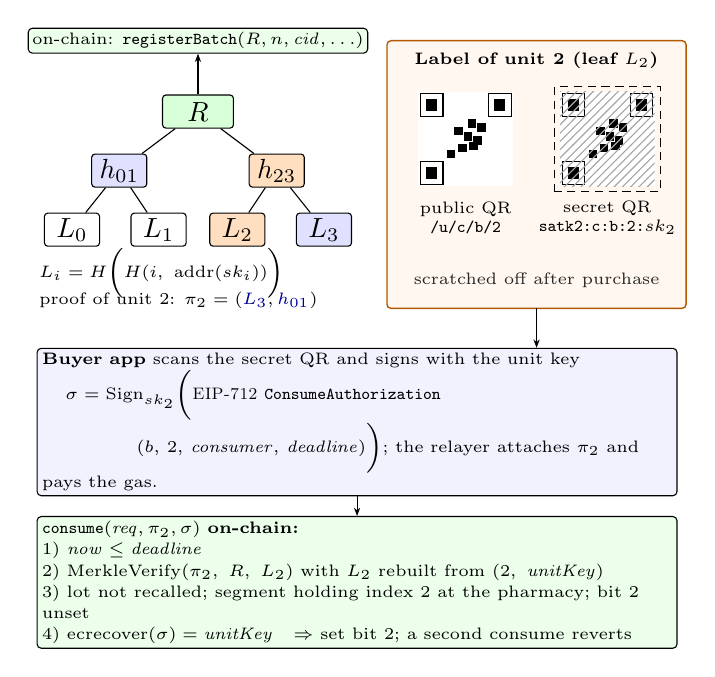
\begin{tikzpicture}[
  x=1mm, y=1mm,
  >={Stealth[length=3pt]},
  hash/.style={draw, rounded corners=1.2pt, minimum width=7mm, minimum height=4.2mm, inner sep=0.8pt, fill=white},
  path/.style={hash, fill=orange!25},
  sib/.style={hash, fill=blue!12},
  lbl/.style={font=\sm, inner sep=0.8pt},
  box/.style={draw, rounded corners=1.5pt, align=left, font=\md, inner sep=1.8pt, text width=80mm},
]
  % ---------------- Merkle tree over the lot
  \node[draw, rounded corners=1.5pt, fill=green!8, lbl, inner sep=1.5pt] (chain) at (20,9)
    {on-chain: \texttt{registerBatch}$(R, n, \mathit{cid}, \dots)$};
  \node[hash, fill=green!15, minimum width=9mm] (root) at (20,0) {$R$};
  \node[sib] (h01) at (10,-7.5) {$h_{01}$};
  \node[path] (h23) at (30,-7.5) {$h_{23}$};
  \node[hash] (l0) at (4,-15) {$L_0$};
  \node[hash] (l1) at (15,-15) {$L_1$};
  \node[path] (l2) at (25,-15) {$L_2$};
  \node[sib] (l3) at (36,-15) {$L_3$};
  \foreach \a/\b in {root/h01, root/h23, h01/l0, h01/l1, h23/l2, h23/l3} \draw (\a) -- (\b);
  \draw[->] (root) -- (chain);
  \node[lbl, anchor=west] at (-0.5,-20.5) {$L_i=H\big(H(i,\ \mathrm{addr}(sk_i))\big)$};
  \node[lbl, anchor=west] at (-0.5,-24) {proof of unit 2: $\pi_2=(\textcolor{blue!60!black}{L_3},\textcolor{blue!60!black}{h_{01}})$};

  % ---------------- two-layer label of unit 2
  \begin{scope}[shift={(63,-6)}]
    \draw[rounded corners=1.5pt, fill=orange!6, draw=orange!70!black, line width=0.5pt] (-19,-19) rectangle (19,15);
    \node[lbl, font=\sm\bfseries] at (0,12.5) {Label of unit 2 (leaf $L_2$)};
    \qr{(-9,2.5)}{12}
    \node[lbl, align=center] at (-9,-7.5) {public QR\\\texttt{/u/c/b/2}};
    \qr{(9,2.5)}{12}
    \fill[pattern=north east lines, pattern color=gray!70] (3,-3.5) rectangle (15,8.5);
    \draw[densely dashed] (2.3,-4.2) rectangle (15.7,9.2);
    \node[lbl, align=center] at (9,-7.5) {secret QR\\\texttt{satk2:c:b:2:}$sk_2$};
    \node[lbl, text=gray!30!black] at (0,-15.5) {scratched off after purchase};
  \end{scope}

  % ---------------- consume
  \node[box, fill=blue!5, anchor=north west] (sig) at (-0.5,-30)
    {\textbf{Buyer app} scans the secret QR and signs with the unit key\\
     \hspace*{3mm}$\sigma=\mathrm{Sign}_{sk_2}\big(\textsc{EIP-712}\ \texttt{ConsumeAuthorization}$\\
     \hspace*{12mm}$(b,\,2,\,\mathit{consumer},\,\mathit{deadline})\big)$;
     the relayer attaches $\pi_2$ and pays the gas.};
  \node[box, fill=green!8, below=2.5mm of sig] (check)
    {\textbf{\texttt{consume}$(\mathit{req},\pi_2,\sigma)$ on-chain:}\\
     1) $\mathit{now}\le\mathit{deadline}$\\
     2) $\mathrm{MerkleVerify}(\pi_2,\ R,\ L_2)$ with $L_2$ rebuilt from $(2,\ \mathit{unitKey})$\\
     3) lot not recalled; segment holding index 2 at the pharmacy; bit 2 unset\\
     4) $\mathrm{ecrecover}(\sigma)=\mathit{unitKey}$\quad$\Rightarrow$ set bit 2; a second consume reverts};
  \draw[->] (63,-25) -- (63,0 |- sig.north);
  \draw[->] (sig) -- (check);
\end{tikzpicture}
\end{document}
